\documentclass[border=5pt]{standalone}
\usepackage{tikz}
\usepackage{tikz-3dplot}
\usetikzlibrary{arrows.meta, 3d, perspective, calc, matrix, positioning}
\usepackage{amsmath}
\begin{document}
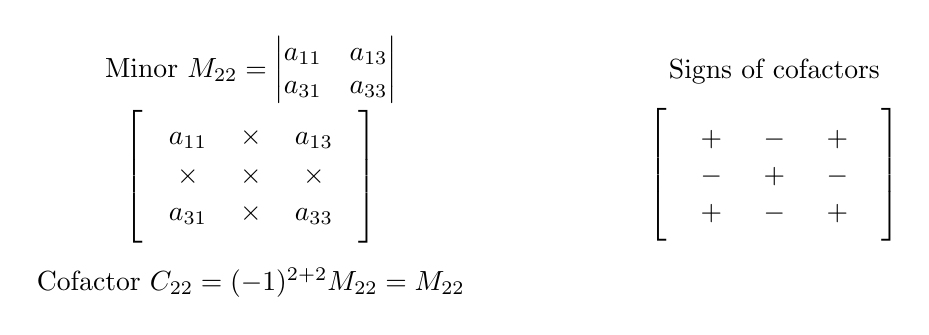
\begin{tikzpicture}

    % Minor explanation
    \matrix (m2) [matrix of math nodes, left delimiter={[}, right delimiter={]}, nodes={minimum width=0.8cm}] {
        a_{11} & \times & a_{13} \\
        \times & \times & \times \\
        a_{31} & \times & a_{33} \\
    };
    \node at ($(m2.north) + (0,0.5)$) {Minor $M_{22} = \begin{vmatrix} a_{11} & a_{13} \\ a_{31} & a_{33} \end{vmatrix}$};

    % Cofactor explanation
    \node at ($(m2.south) + (0,-0.5)$) {Cofactor $C_{22} = (-1)^{2+2} M_{22} = M_{22}$};

    % Minor explanation
    \matrix (m3) [matrix of math nodes, left delimiter={[}, right delimiter={]}, right=4cm of m2, nodes={minimum width=0.8cm}] {
        + & - & + \\
        - & + & - \\
        + & - & + \\
    };
    \node at ($(m3.north) + (0,0.5)$) {Signs of cofactors};

\end{tikzpicture}
\end{document}
